\part{长度与比例}

\begin{exercise}
    (香港 1998) 设 $PQRS$ 是圆内接四边形,$\angle PSR = 90^\circ$,且 $H, K$ 分别是 $Q$ 到直线 $PR, PS$ 的高的垂足。证明 $HK$ 平分 $QS$。
\end{exercise}
\begin{figure}[H]
    \centering
    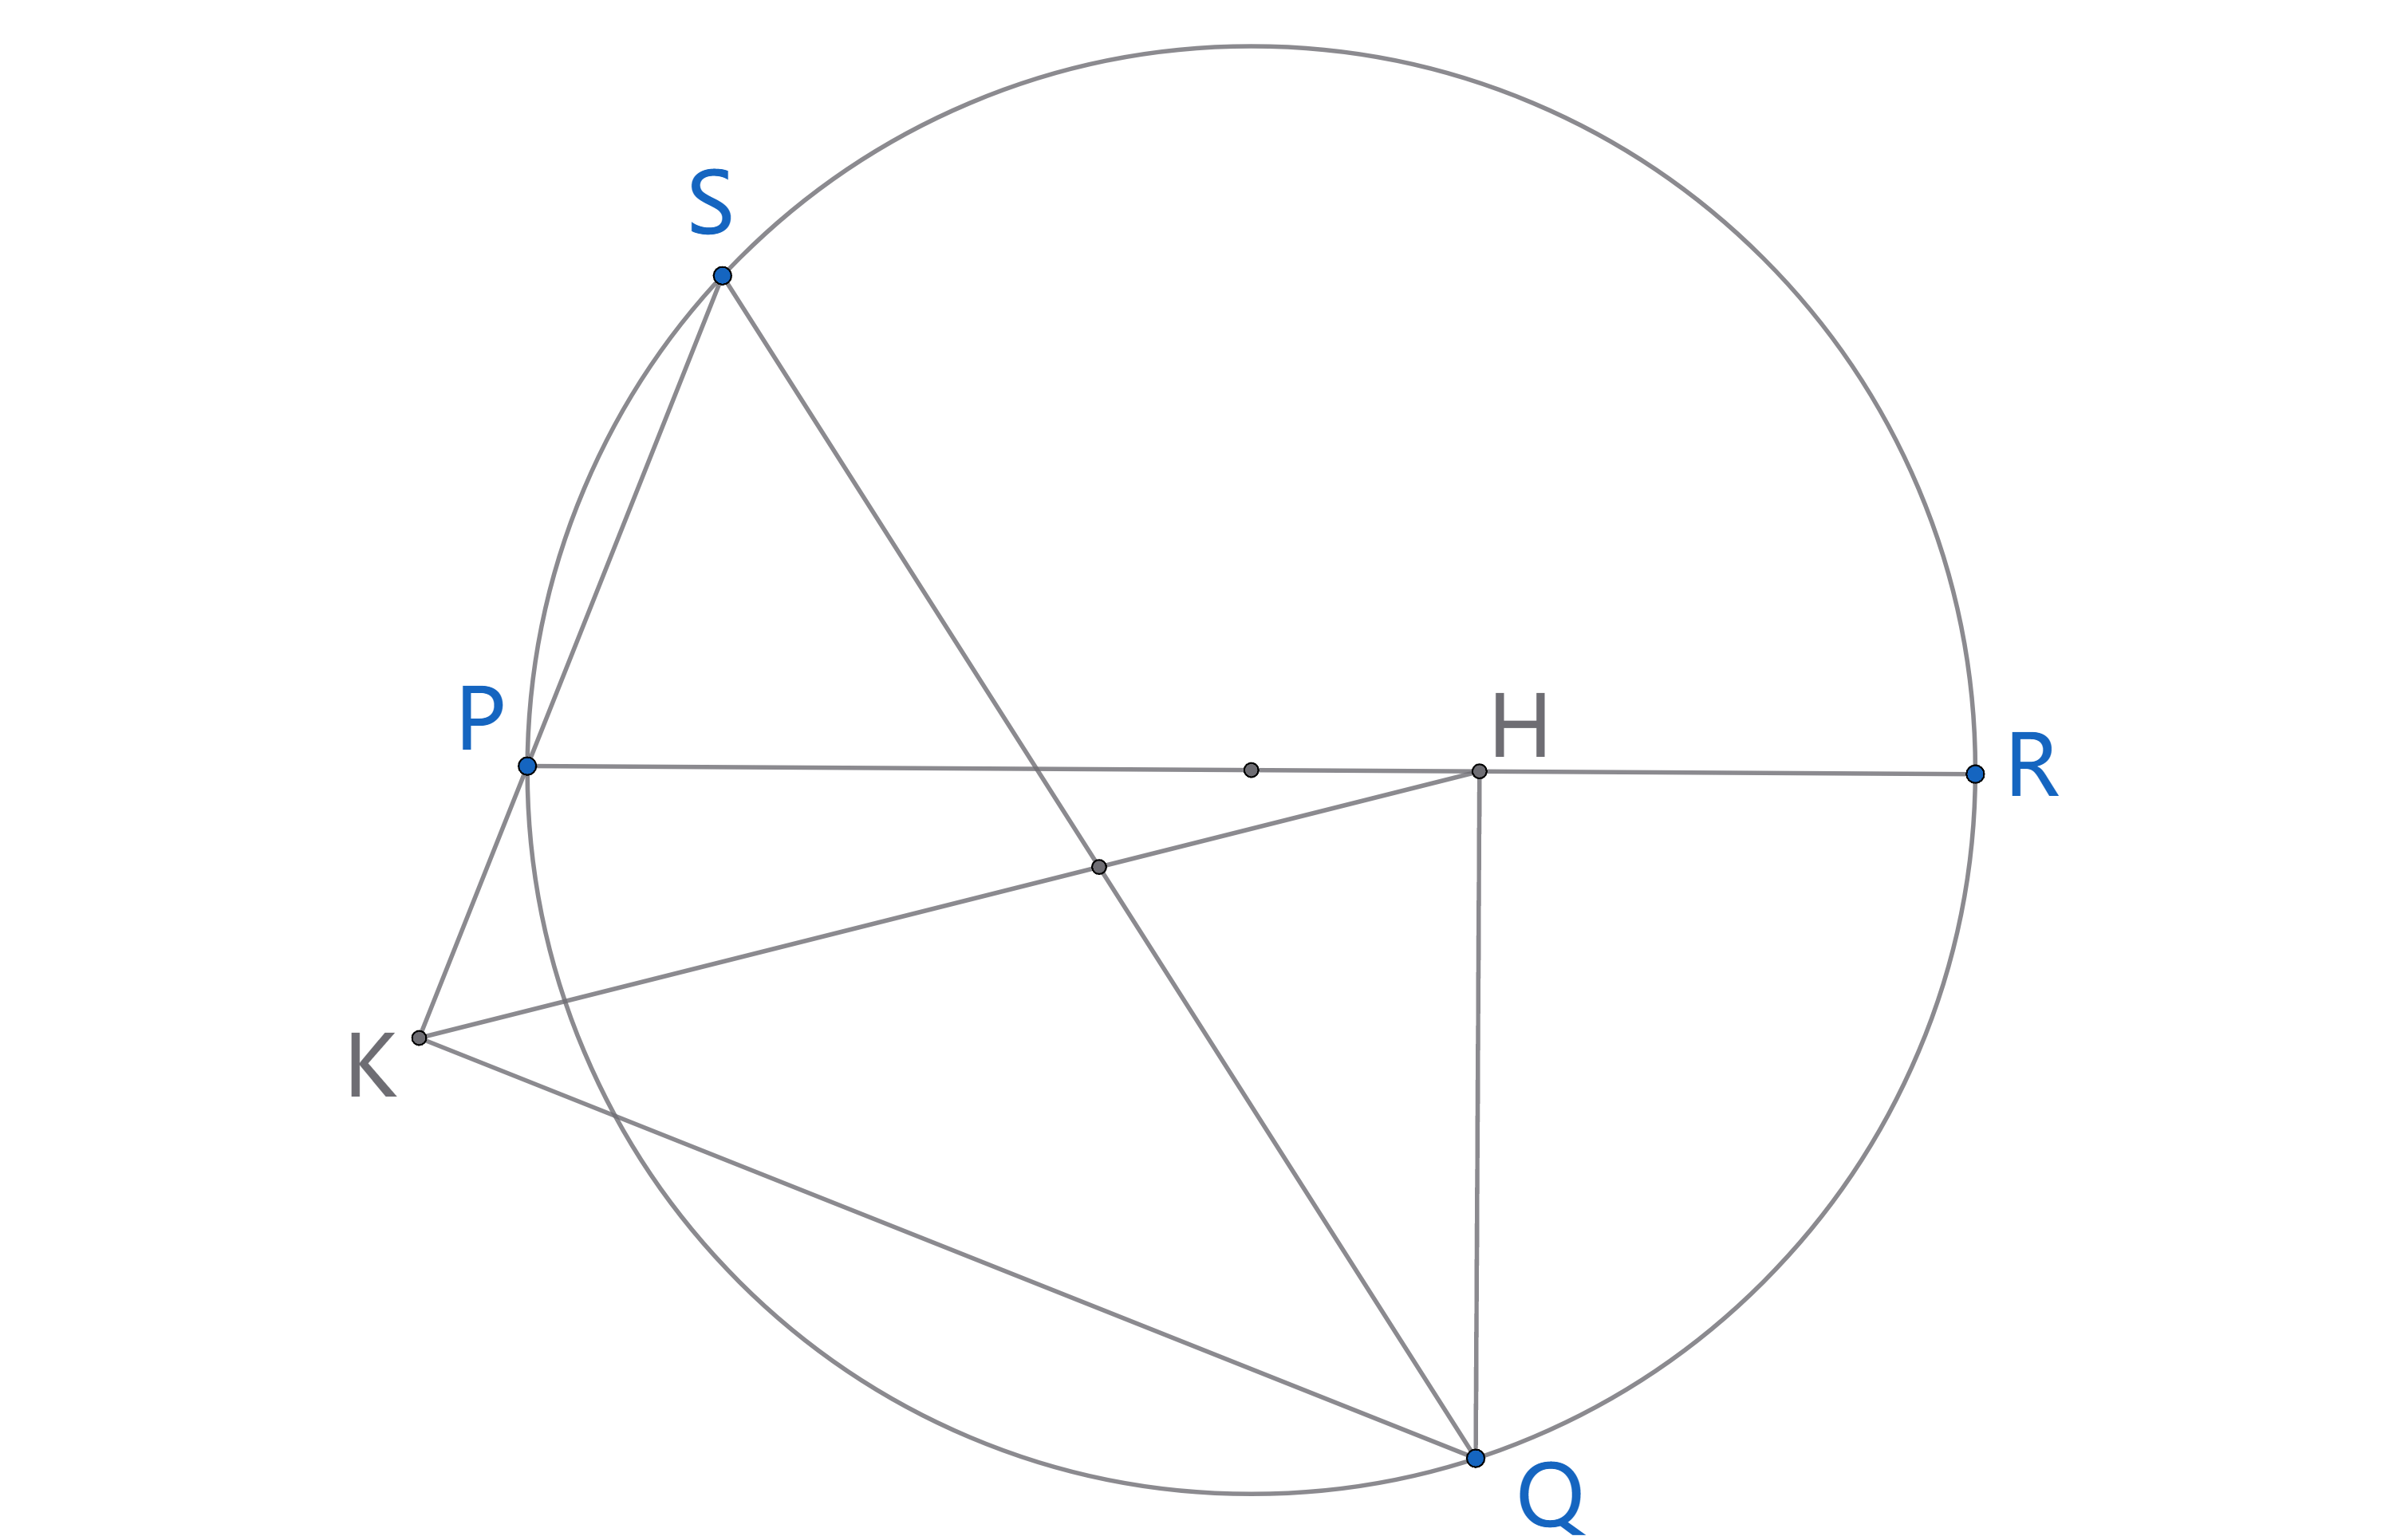
\includegraphics[width=0.7\linewidth]{figures/exercises/441.png}
\end{figure}


\begin{exercise}
    (USAMO 1988/4) 设 $\triangle ABC$ 的内心是 $I$。证明:$\triangle IAB, \triangle IBC, \triangle ICA$ 的外心所在的圆必是 $\triangle ABC$ 的外心。
\end{exercise}
\begin{figure}[H]
    \centering
    \includegraphics[width=0.7\linewidth]{figures/exercises/442.png}
\end{figure}


%-----------------------------------
\newpage 
\begin{exercise}
    (USAMO 1995/3) 给定不等边、非直角 $\triangle ABC$,设 $O$ 是外心,$A_1, B_1, C_1$ 分别是 $\overline{BC}, \overline{CA}, \overline{AB}$ 的中点。点 $A_2$ 在射线 $OA_1$ 上,使得 $\triangle OAA_1$ 和 $\triangle OA_2A$ 相似。点 $B_2, C_2$ 分别在射线 $OB_1, OC_1$ 上类似地定义。证明:$AA_2, BB_2, CC_2$ 三线共点。
\end{exercise}
\begin{figure}[H]
    \centering
    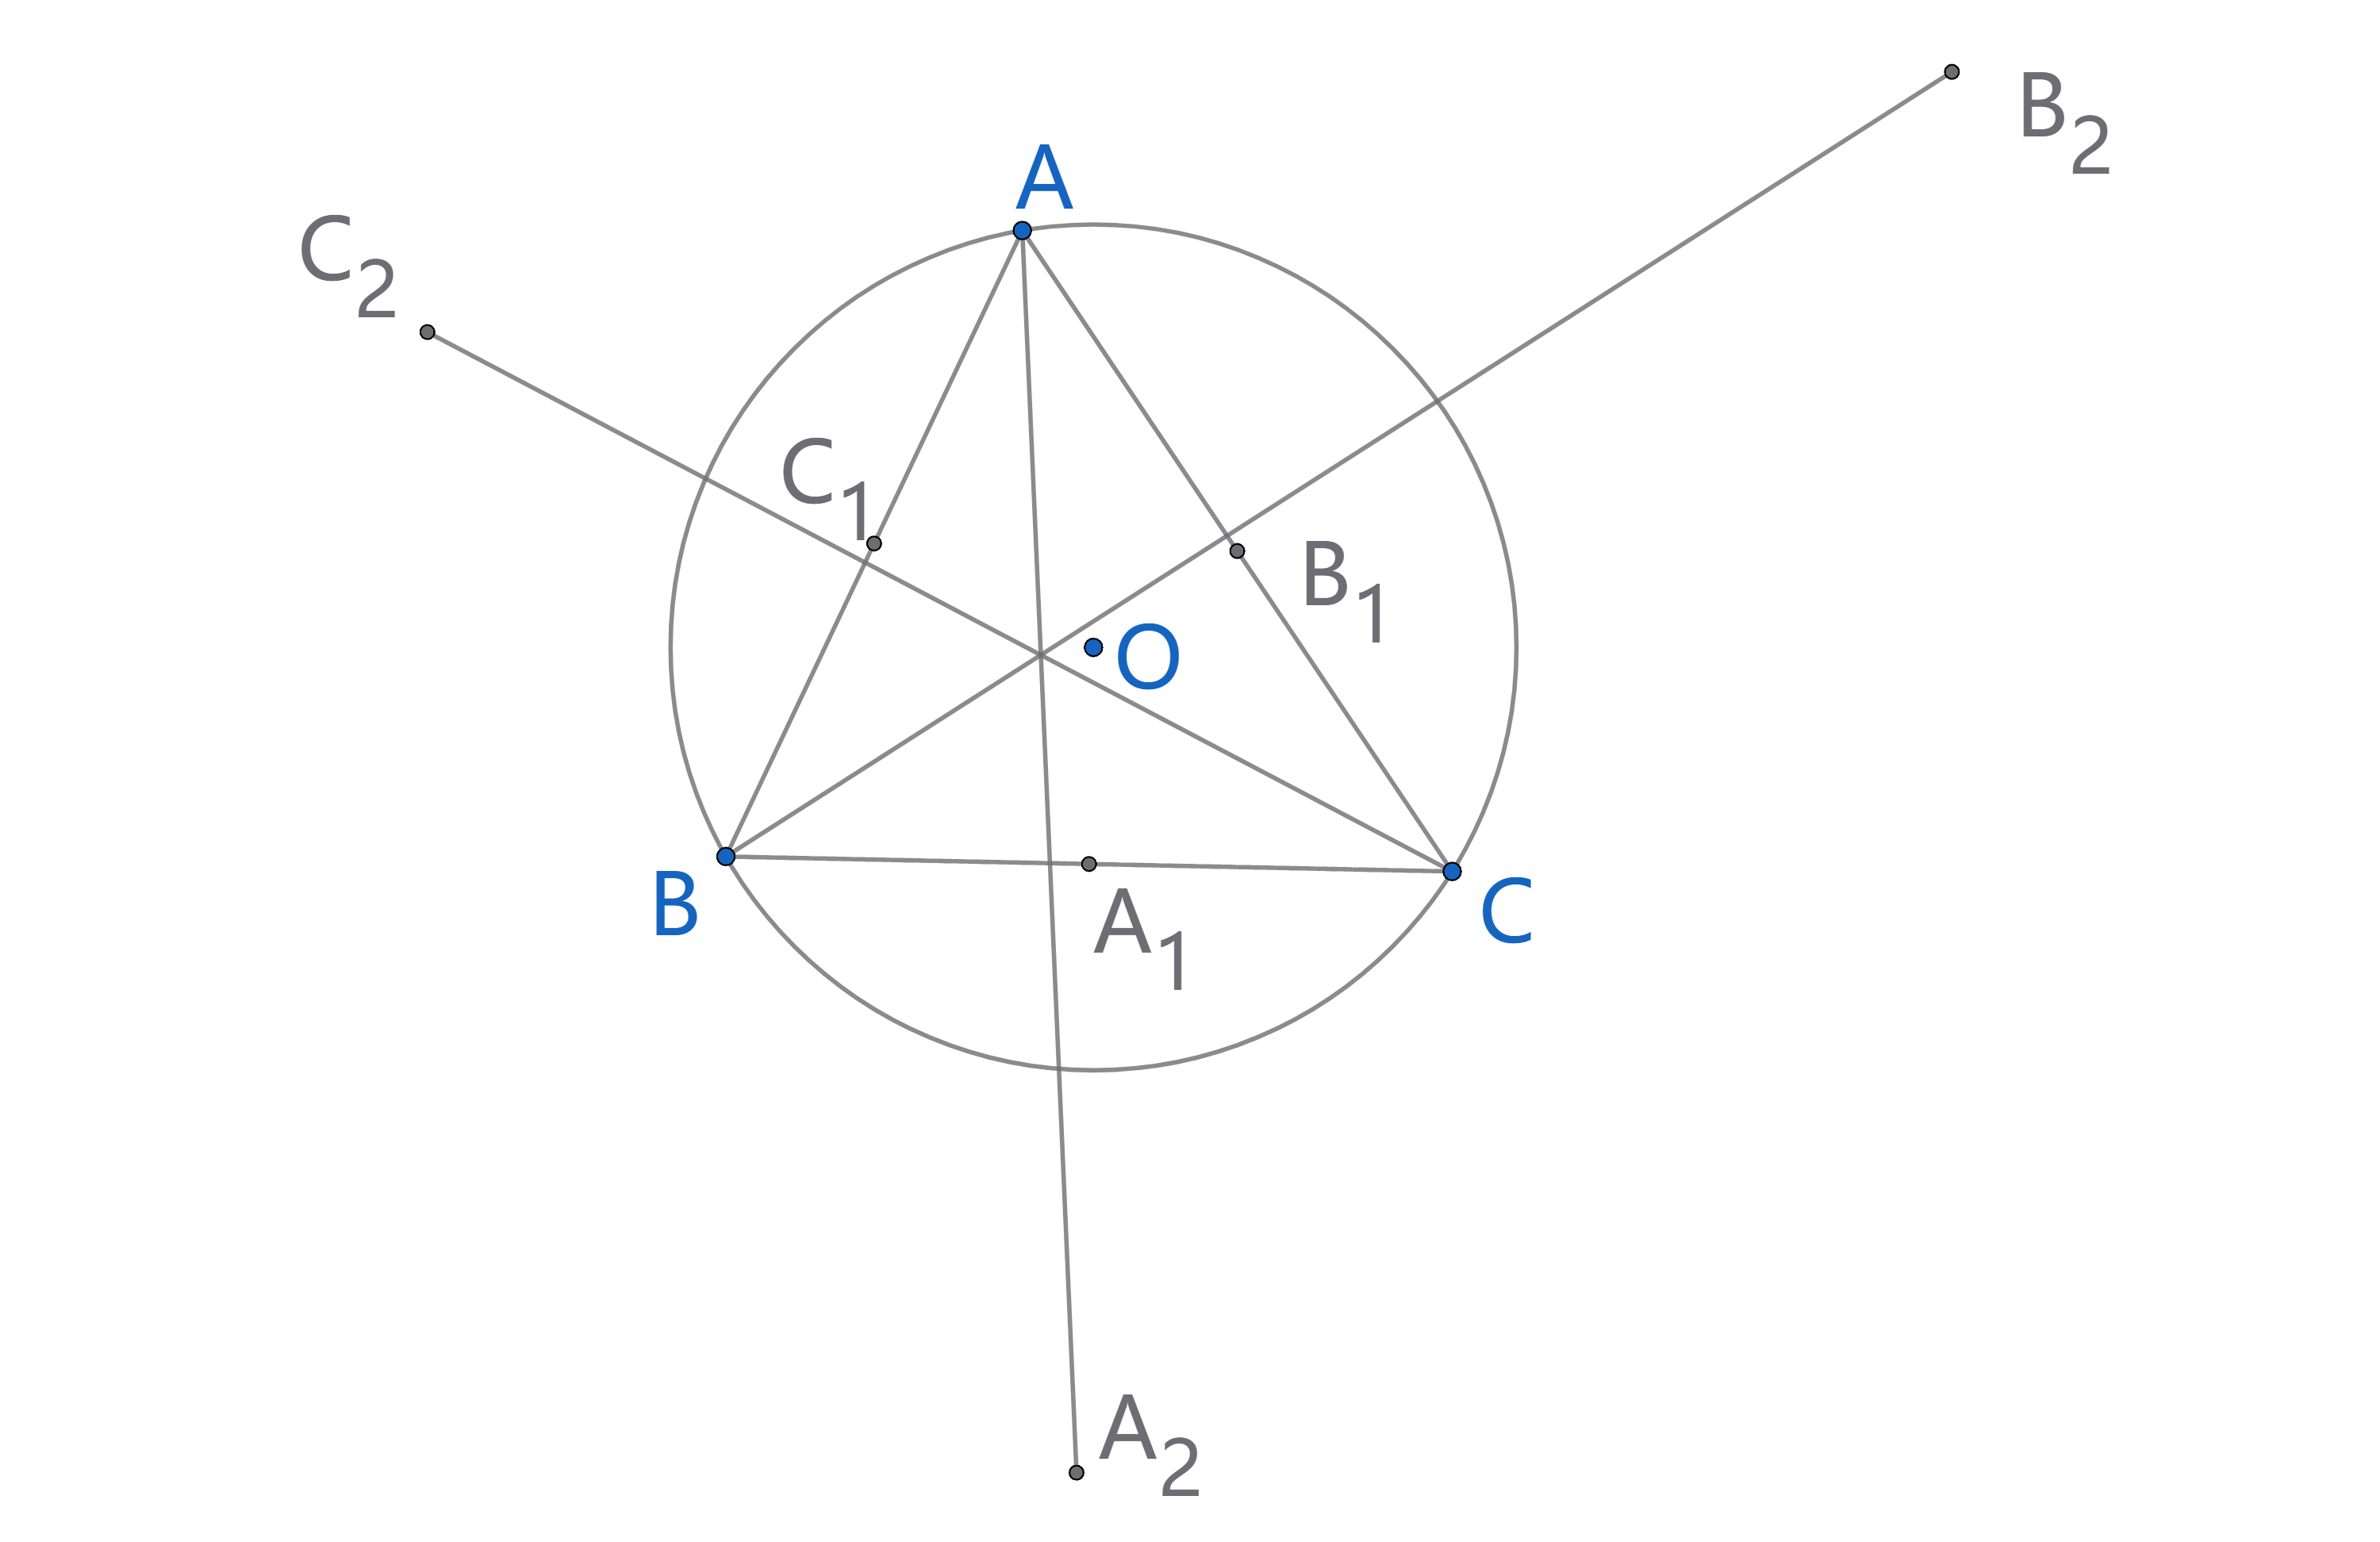
\includegraphics[width=0.7\linewidth]{figures/exercises/443.png}
\end{figure}


\begin{exercise}
    (USATST 2014) 设 $\triangle ABC$ 是一个锐角三角形,$X$ 是劣弧 $\overarc{BC}$ 上的动点。设 $P, Q$ 分别是 $X$ 到直线 $CA, CB$ 的投影。设 $R$ 是直线 $PQ$ 与 $B$ 到 $AC$ 的垂线的交点。设直线 $l$ 经过 $P$ 平行于 $\overline{XR}$。证明:当 $X$ 在劣弧 $\overarc{BC}$ 上变动时,直线 $l$ 总是经过一个定点。
\end{exercise}
\begin{figure}[H]
    \centering
    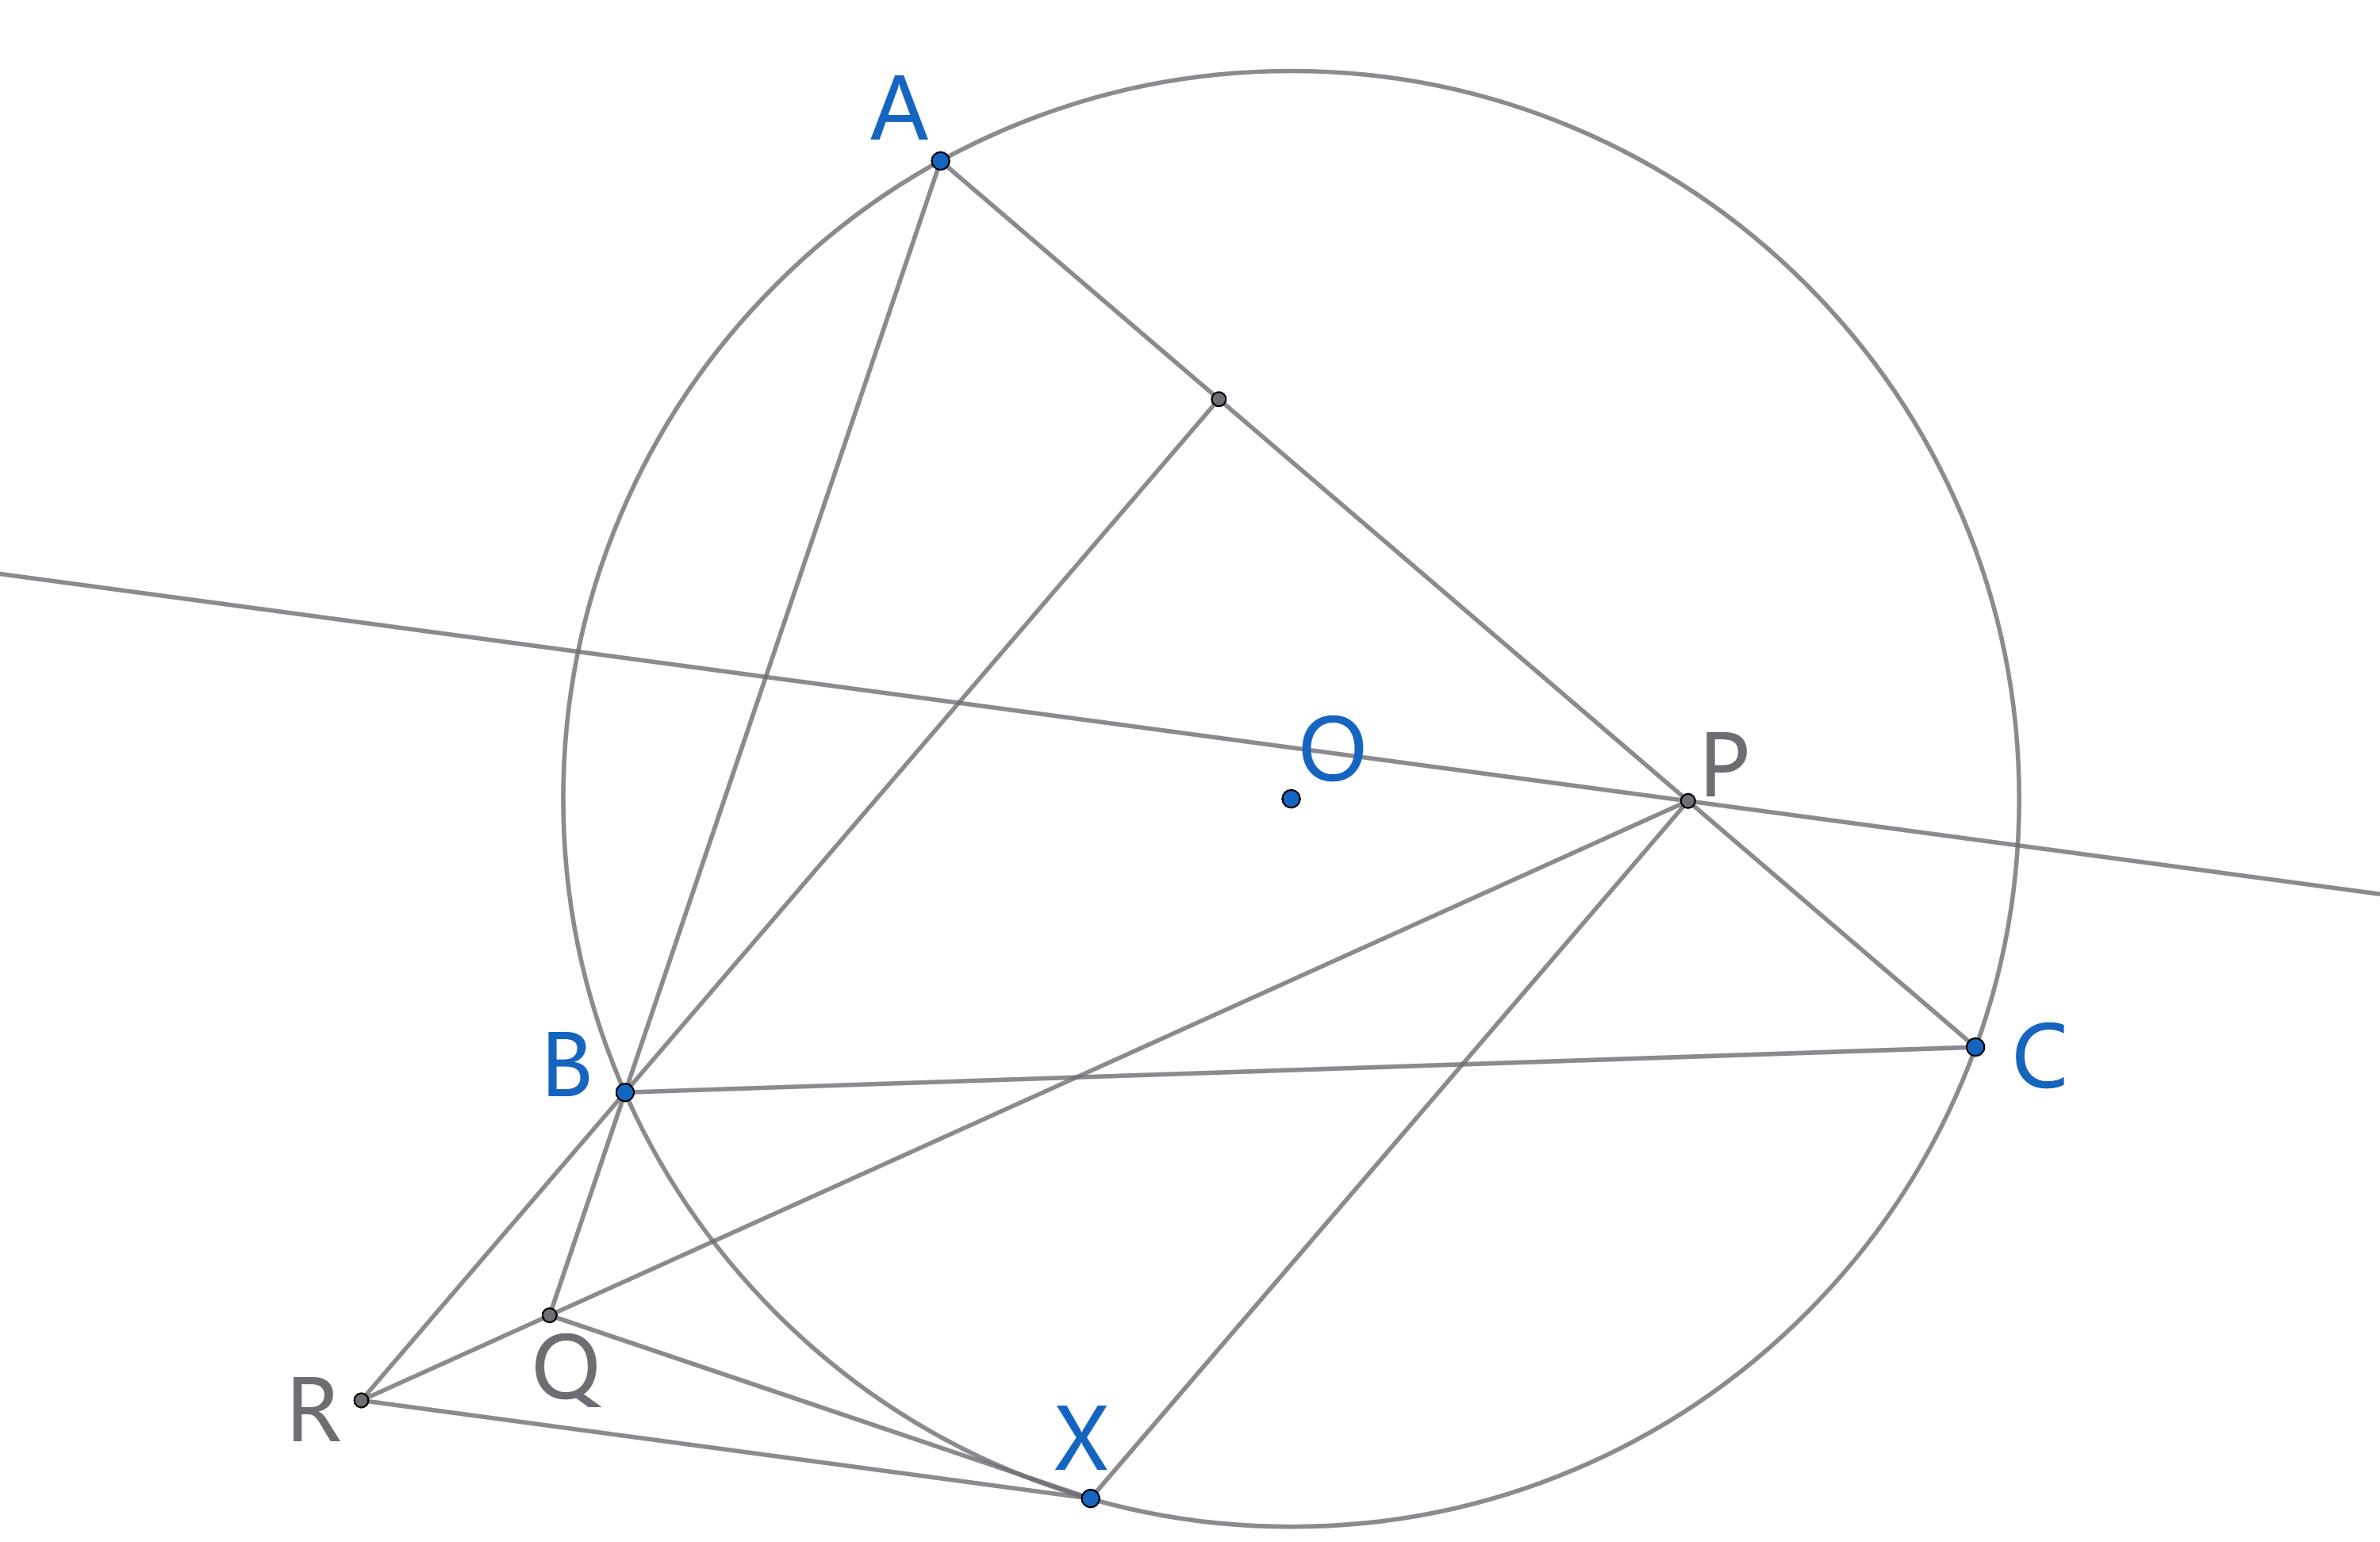
\includegraphics[width=0.7\linewidth]{figures/exercises/444.png}
\end{figure}


%-----------------------------------
\newpage 
\begin{exercise}
    (USATST 2011/1) 在锐角 $\triangle ABC$ 中,$D, E, F$ 分别是 $BC, CA, AB$ 上的高的垂足,$H$ 是垂心。点 $P, Q$ 在线段 $EF$ 上,满足 $AP \perp EF, HQ \perp EF$。直线 $DP$ 和 $QH$ 相交于 $R$。计算 $\frac{HQ}{HR}$。
\end{exercise}
\begin{figure}[H]
    \centering
    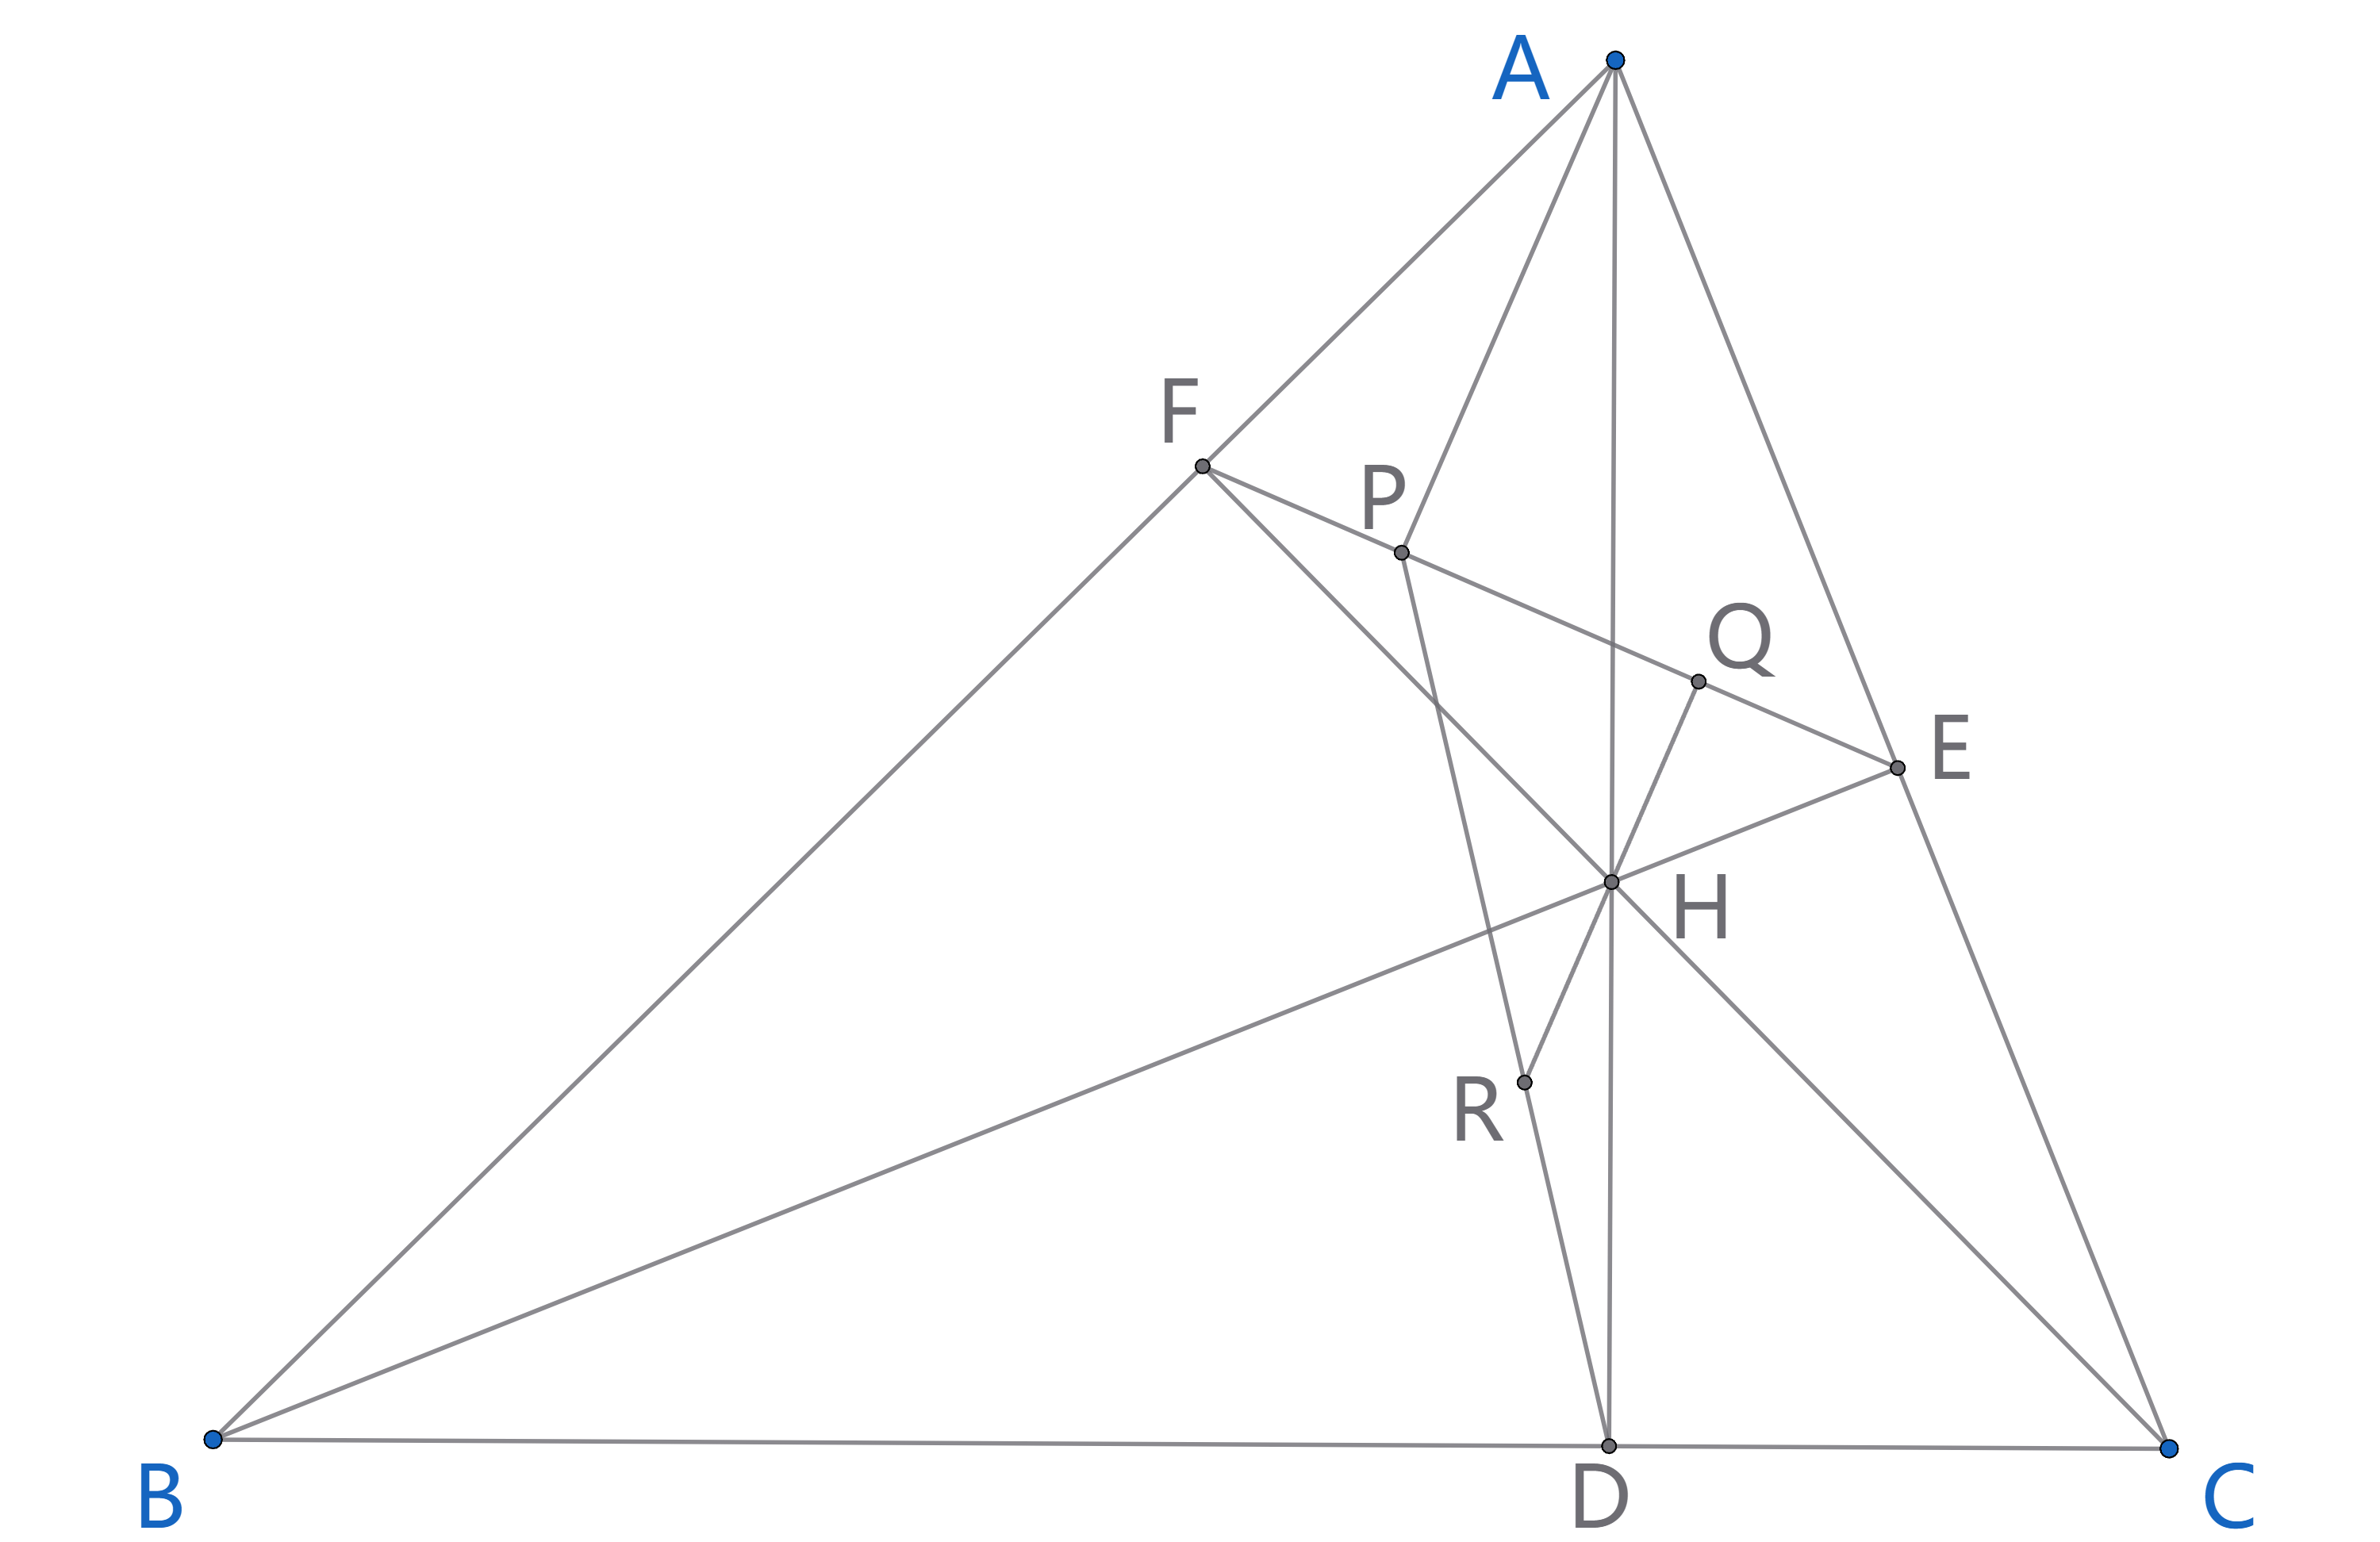
\includegraphics[width=0.7\linewidth]{figures/exercises/445.png}
\end{figure}

\begin{exercise}
    (ELMO 预选题 2012) 圆 $\Omega, \omega$ 内切于 $C$, $\Omega$ 的弦 $AB$ 与 $\omega$ 相切于 $\overline{AB}$ 的中点 $E$,另一个圆 $\omega_1$ 与 $\Omega, \omega, \overline{AB}$ 分别相切于 $D, Z, F$,射线 $CD, AB$ 相交于 $P$。若 $M \neq C$ 是优弧 $\overarc{AB}$ 的中点,证明:$\tan \angle ZEP = \frac{PE}{CM}$。
\end{exercise}
\begin{figure}[H]
    \centering
    \includegraphics[width=0.7\linewidth]{figures/exercises/446.png}
\end{figure}


%-----------------------------------
\newpage 
\begin{exercise}
    (USAMO 2011/5) 设 $P$ 是凸四边形 $ABCD$ 内一点,点 $Q_1, Q_2$ 在 $ABCD$ 的内部,满足 $\angle Q_1BC = \angle ABP$,$\angle Q_1CB = \angle DCP$,$\angle Q_2AD = \angle BAP$,$\angle Q_2DA = \angle CDP$。证明:$Q_1Q_2 \parallel AB \iff Q_1Q_2 \parallel CD$。
\end{exercise}
\begin{figure}[H]
    \centering
    \includegraphics[width=0.7\linewidth]{figures/exercises/447.png}
\end{figure}

\begin{exercise}
    (日本 2009) $\triangle ABC$ 内接于圆 $\Gamma$,以 $O$ 为圆心的圆与 $BC$ 相切于 $P$,与不包含 $A$ 的 $\overset{\frown}{BC}$ 内切于 $Q$。证明:若 $\angle BAO = \angle CAO$,则 $\angle PAO = \angle QAO$。
\end{exercise}
\begin{figure}[H]
    \centering
    \includegraphics[width=0.7\linewidth]{figures/exercises/448.png}
\end{figure}


%-----------------------------------
\newpage 
\begin{exercise}
    设 $\triangle ABC$ 的内切圆与 $BC$ 相切于 $D$。设 $T$ 是 $A$-伪内切圆与 $(ABC)$ 的切点。证明:$\angle BTA = \angle CTD$。
\end{exercise}
\begin{figure}[H]
    \centering
    \includegraphics[width=0.7\linewidth]{figures/exercises/449.png}
\end{figure}

\begin{exercise}
    (越南 TST 2003/2) 设不等边 $\triangle ABC$ 的外心为 $O$,内心为 $I$。设 $H, K, L$ 分别是从 $A, B, C$ 引出的三条高的垂足。记高 $AH, BK, CL$ 的中点分别是 $A_0, B_0, C_0$。$\triangle ABC$ 的内切圆与 $BC, CA, AB$ 分别相切于 $D, E, F$。证明:四条直线 $A_0D, B_0E, C_0F$ 和 $OI$ 共点。
\end{exercise}
\begin{figure}[H]
    \centering
    \includegraphics[width=0.7\linewidth]{figures/exercises/450.png}
\end{figure}


%-----------------------------------
\newpage 
\begin{exercise}
    (Sharygin 2013) $\triangle ABC$ 的内切圆分别与 $BC, CA, AB$ 相切于 $D, E, F$。从 $I$ 到 $C$-中线的垂线与直线 $DE$ 相交于 $K$。证明:$\overline{CK} \parallel AB$。
\end{exercise}
\begin{figure}[H]
    \centering
    \includegraphics[width=0.7\linewidth]{figures/exercises/451.png}
\end{figure}

\begin{exercise}
    (APMO 2012/4) 设锐角 $\triangle ABC$ 中,从点 $A$ 出发的高的垂足是 $D$,$M$ 是 $BC$ 的中点,$H$ 是 $\triangle ABC$ 的垂心。设射线 $MH$ 与 $(ABC)$ 交于 $E$,直线 $ED$ 与 $(ABC)$ 交于不同于 $E$ 的点 $F$。证明:$\frac{BF}{CF} = \frac{AB}{AC}$。
\end{exercise}
\begin{figure}[H]
    \centering
    \includegraphics[width=0.7\linewidth]{figures/exercises/452.png}
\end{figure}


\begin{exercise}
    (预选题 2002/G7) 锐角 $\triangle ABC$ 的内切圆 $\Omega$ 与 $\overline{BC}$ 相切于 $K$。设 $AD$ 是 $\triangle ABC$ 的高,$M$ 是 $\overline{AD}$ 的中点。若 $N$ 是直线 $KM$ 与 $\Omega$ 的交点(不同于 $K$),证明:$\Omega$ 与 $(BCN)$ 相切于 $N$。
\end{exercise}
\begin{figure}[H]
    \centering
    \includegraphics[width=0.7\linewidth]{figures/exercises/453.png}
\end{figure}